\documentclass[../main.tex]{subfile}
\begin{document}
    \section{How to use} This plugin has 4 main components to use. Two of them are core components and the other two are cosmetics.
    \begin{figure}[H]
        \centering
        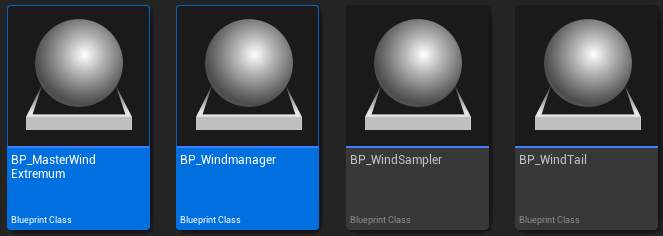
\includegraphics[width=.5\textwidth]{Ressources/Files.png}
        \caption{The four relevant components. The two outlined are the core components and the other one are cosmetics.}
    \end{figure}
    \begin{itemize}
        \item[0] Download a ZIP of the repo and cut past the folder content at the same location than your content folder.
         This is important to do carefully to avoid any issue with the references.
        \item[1] Place the extrema where you want to and define them as boosters, wells or sources. You can play with their influence strength.
        \begin{figure}[H]
            \centering
            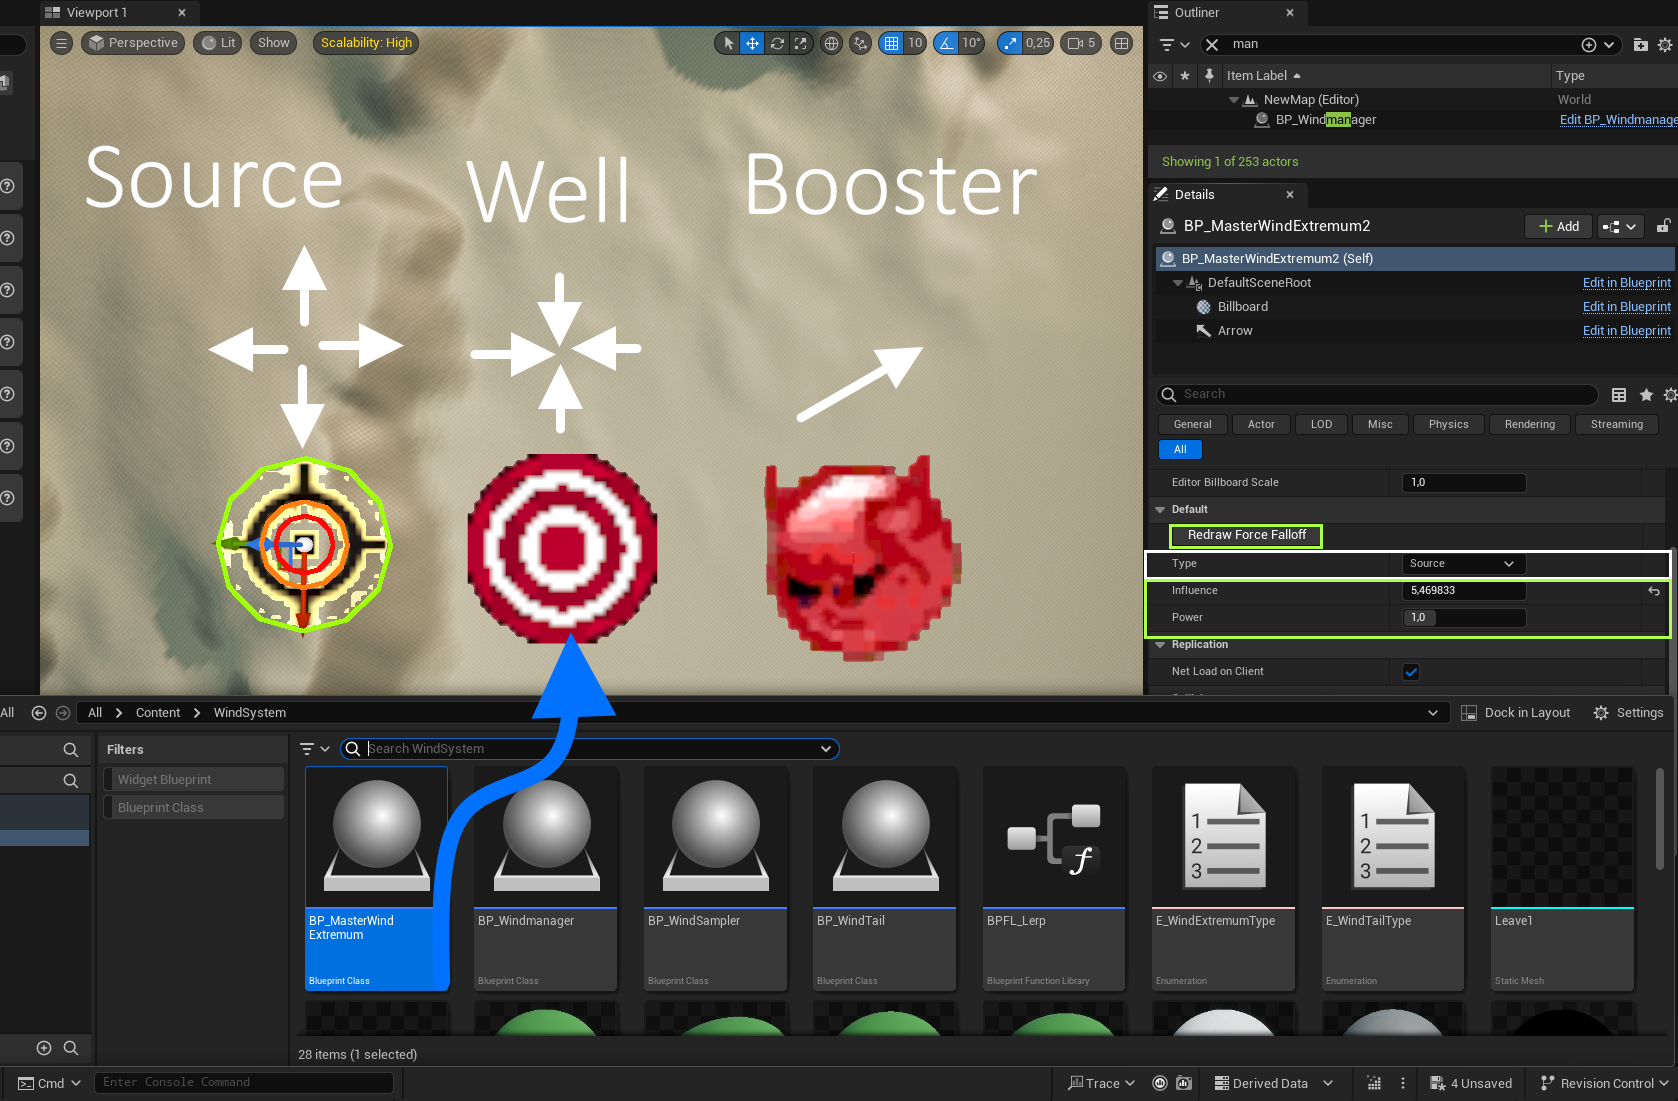
\includegraphics[width=1\textwidth]{Ressources/WindExtrema.png}
            \caption{The three types of extremas. The green, orange and yellow debug circles gie you the radius at wich wr have 25, 50 and 75\% of the influence.}
        \end{figure}
        \item[2] Place the wind manager an store the wind extrema inside the array. Redraw and reshape updates the shaders.
        \begin{figure}[H]
            \centering
            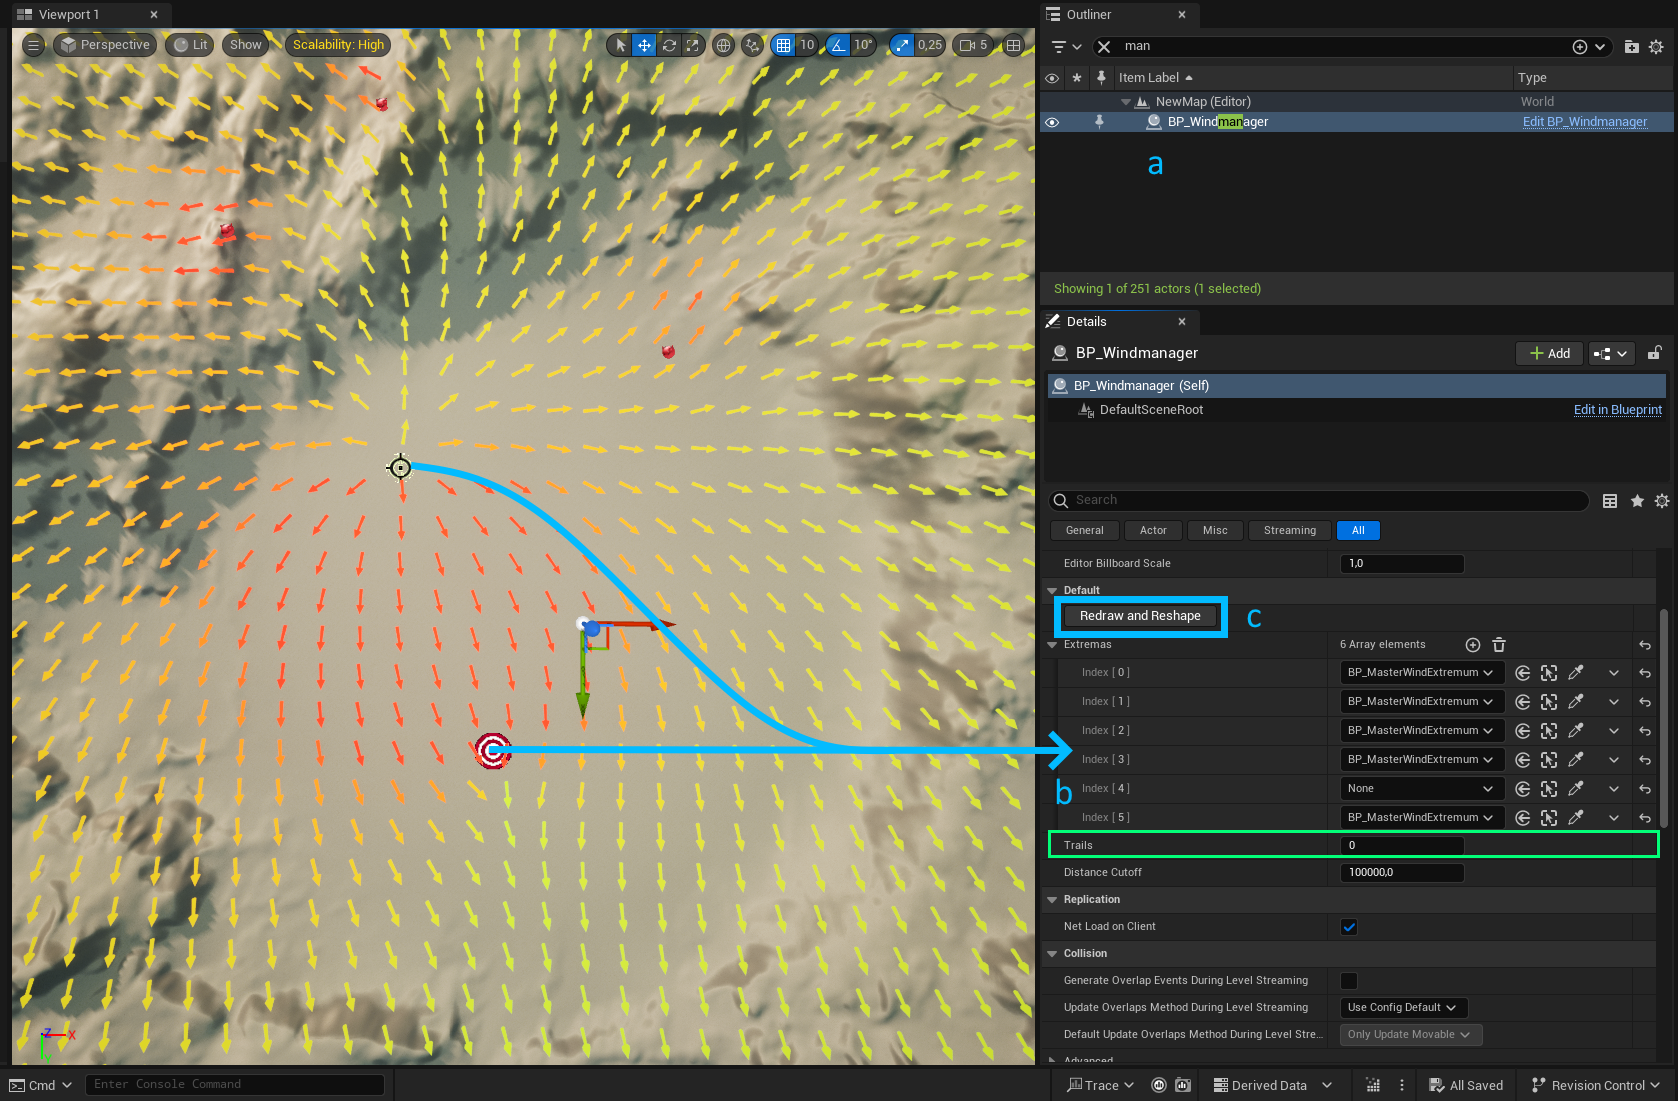
\includegraphics[width=1\textwidth]{Ressources/WindManager.png}
            \caption{The wind manager. The green parameter stays how much wind tails will spawn arround the player.}
        \end{figure}
        \item[3] Let the system know about the size of the world so it can correctly map the wind deformation to the trees. 
        To do, this give the side length of the world to the material parameter collection \texttt{MP\_Wind}.
        \begin{figure}[H]
            \centering
            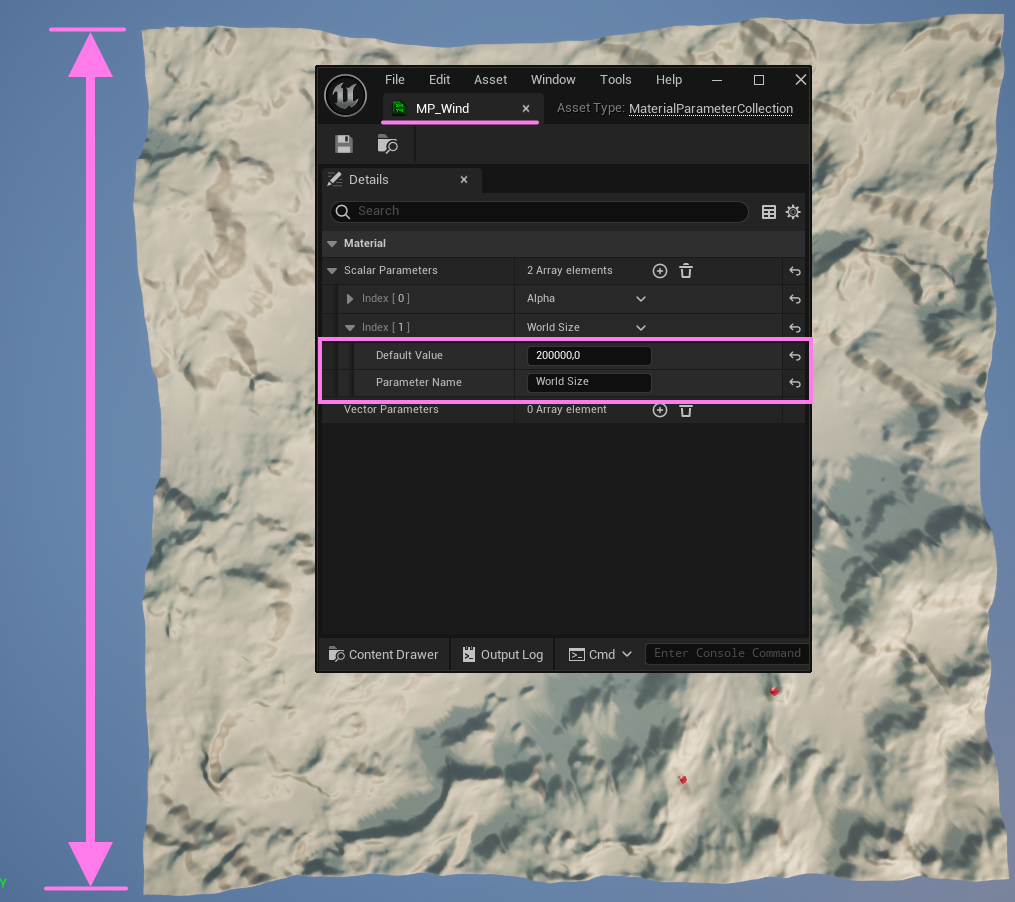
\includegraphics[width=1\textwidth]{Ressources/WorldSize.png}
            \caption{The parameter collection to let the system now about the world size.}
        \end{figure}
        \item[4] Debug the wind using the wind sampler tool. Define a grid resolution and, and a spacement. Specify the wind manager to make to computations.
        \begin{figure}[H]
            \centering
            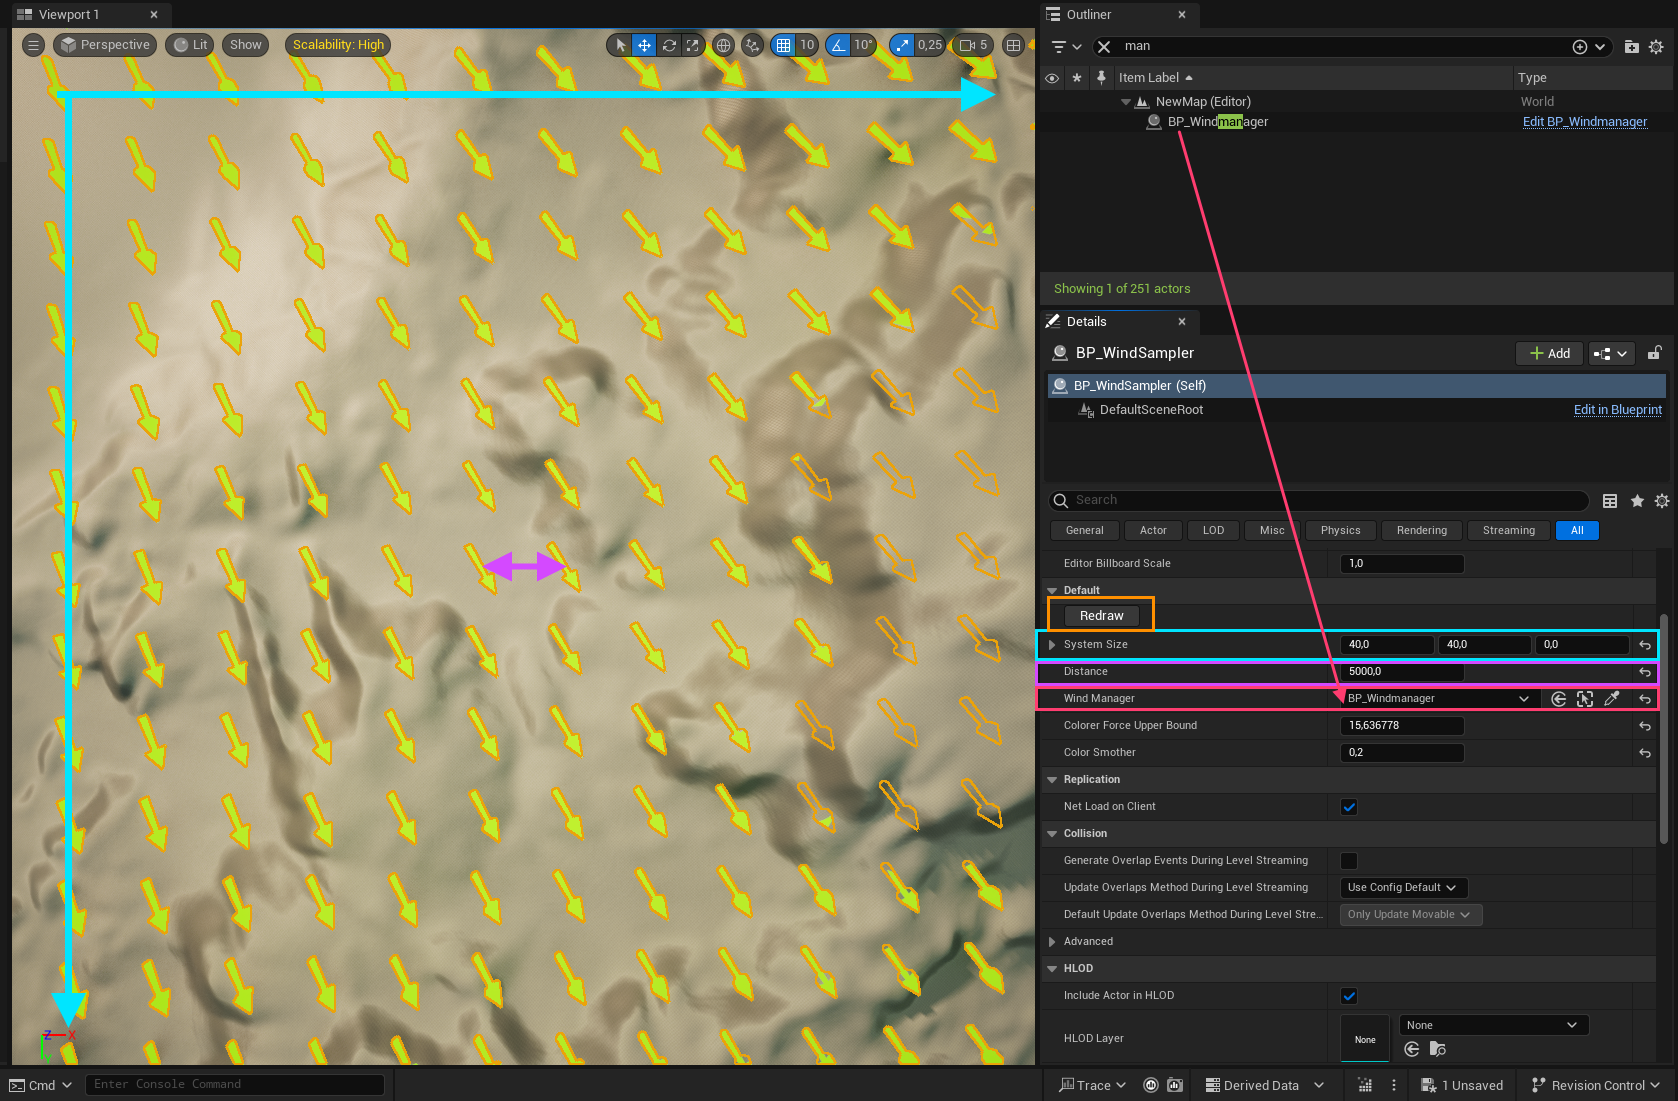
\includegraphics[width=1\textwidth]{Ressources/WindSampler.png}
            \caption{The wind sampler tool. Please reference the wind manager or this wont work properly.}
        \end{figure}
        \item[5] Use the \texttt{Dynamic Wind} matieral function in your folliage.
        \begin{figure}[H]    
            \centering
            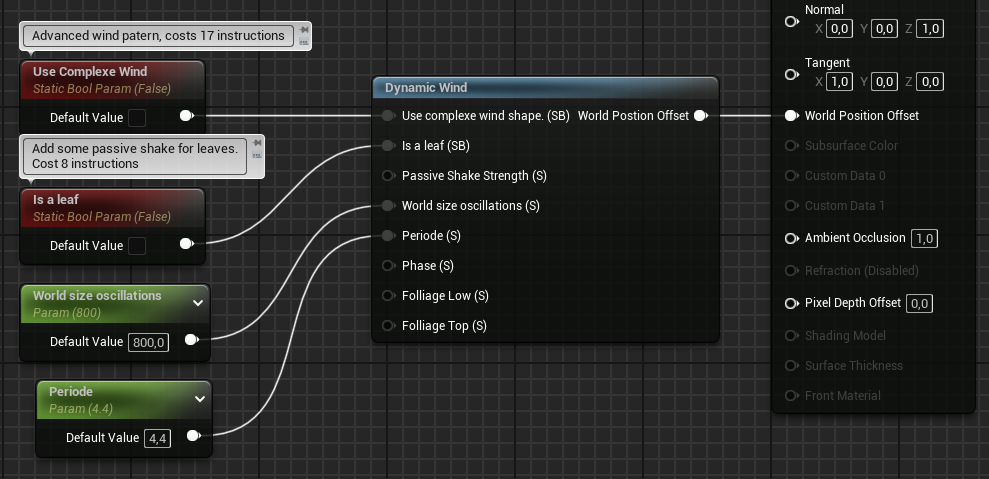
\includegraphics[width=.75\textwidth]{Ressources/MaterialInstance.png}
            \caption{The use of the materal function.}
        \end{figure}
    \end{itemize}

    An there we have it! The tail respawn after a while. To desactivate the trace on spawn, please search the event \texttt{RetraceAtSpawn}
     in \texttt{BP\_WindTail} and naviagte to the node \texttt{Line Trace By Channel}. There, set the \texttt{Draw Debug mode} to none.
   
\end{document}